\newcommand{\QpuDocTitle}{QPU Language Reference}
\newcommand{\QpuDocSubtitle}{Complete Protocol and Truth-Table Syntax}
\newcommand{\QpuHeaderTitle}{Language Reference}
\newcommand{\QpuDocDescription}{%
The exact QPU protocol surface: references, constants, flags, gates, process
composition, truth-table metadata, compatibility behavior, diagnostics, and
quick-reference grammar.
}
\documentclass[10pt,letterpaper]{article}

% Stable output supports docs:check even when translation uses a temporary directory.
\ifdefined\pdftrailerid
  \pdftrailerid{}
\fi

\usepackage[T1]{fontenc}
\usepackage[utf8]{inputenc}
\usepackage{lmodern}
\usepackage[margin=0.72in]{geometry}
\usepackage{amsmath,amssymb,mathtools}
\usepackage{booktabs,longtable,tabularx,array}
\usepackage[dvipsnames,table]{xcolor}
\usepackage{listings}
\usepackage{tikz}
\usepackage{enumitem}
\usepackage{fancyhdr}
\usepackage{microtype}
\usepackage[hidelinks]{hyperref}
\usepackage{bookmark}
\usepackage{titlesec}

\usetikzlibrary{arrows.meta,calc,positioning}

\definecolor{QpuNavy}{HTML}{0F172A}
\definecolor{QpuBlue}{HTML}{2563EB}
\definecolor{QpuCyan}{HTML}{0891B2}
\definecolor{QpuGreen}{HTML}{047857}
\definecolor{QpuAmber}{HTML}{B45309}
\definecolor{QpuRed}{HTML}{B91C1C}
\definecolor{QpuPaper}{HTML}{F8FAFC}
\definecolor{QpuLine}{HTML}{CBD5E1}
\definecolor{CodeBg}{HTML}{F1F5F9}
\definecolor{CodeComment}{HTML}{64748B}

\providecommand{\QpuDocTitle}{QPU Documentation}
\providecommand{\QpuDocSubtitle}{System Guide}
\providecommand{\QpuDocDescription}{A guide to the QPU circuit system.}
\providecommand{\QpuHeaderTitle}{QPU Documentation}

\hypersetup{
  pdftitle={\QpuDocTitle: \QpuDocSubtitle},
  pdfauthor={Bailey Forbes},
  pdfsubject={QPU protocol syntax, quantum gates, mathematics, and truth tables},
  pdfkeywords={QPU, quantum circuit, protocol, system syntax, truth table}
}

\pagestyle{fancy}
\fancyhf{}
\lhead{\textcolor{QpuNavy}{QPU Circuit Compiler}}
\rhead{\textcolor{QpuNavy}{\QpuHeaderTitle}}
\cfoot{\thepage}
\renewcommand{\headrulewidth}{0.3pt}

\titleformat{\section}{\Large\bfseries\color{QpuNavy}}{\thesection}{0.55em}{}
\titleformat{\subsection}{\large\bfseries\color{QpuBlue}}{\thesubsection}{0.5em}{}
\titleformat{\subsubsection}{\normalsize\bfseries\color{QpuCyan}}{\thesubsubsection}{0.45em}{}
\setlist{nosep,leftmargin=1.5em}
\setlength{\parindent}{0pt}
\setlength{\parskip}{4pt}
\setlength{\tabcolsep}{4pt}
\renewcommand{\arraystretch}{1.15}

\lstdefinelanguage{QPU}{
  morekeywords={
    PARAMS,MAIN-PROCESS,INCREASECYCLE,COMPILEPROCESS,FREE,SET,JOIN,SPLIT,
    CALL,DECLARECHILD,RUNCHILD,REC,TREC,RECUR,EXIT,IF,ELSE,ENDIF,RETURNVALS,ACCEPTVALS,MASTERVAL,SAVE_STATE,
    LOAD_STATE,CREATETOKEN,DELETETOKEN,X,Y,Z,H,S,T,CNOT,CCNOT,CZ,CY,
    SWAP,PHASE,RX,RY,RZ,CPHASE,MEASURE,NOT,AND,NAND,OR,XOR
  },
  sensitive=false,
  morecomment=[l]{\#},
  morecomment=[s]{/*}{*/},
  morestring=[b]"
}
\lstset{
  language=QPU,
  basicstyle=\ttfamily\small,
  keywordstyle=\bfseries\color{QpuBlue},
  commentstyle=\itshape\color{CodeComment},
  backgroundcolor=\color{CodeBg},
  frame=single,
  rulecolor=\color{QpuLine},
  framerule=0.4pt,
  xleftmargin=0.4em,
  framexleftmargin=0.35em,
  columns=fullflexible,
  keepspaces=true,
  showstringspaces=false,
  breaklines=true,
  aboveskip=5pt,
  belowskip=5pt
}

\newcommand{\code}[1]{\texttt{\detokenize{#1}}}
\newcommand{\ket}[1]{\lvert #1\rangle}
\newcommand{\bra}[1]{\langle #1\rvert}
\newcommand{\status}[1]{\textsf{\small #1}}
\newcommand{\implemented}{\textcolor{QpuGreen}{\status{lowered/executed}}}
\newcommand{\acceptedonly}{\textcolor{QpuAmber}{\status{accepted, not executed}}}
\newcommand{\internal}{\textcolor{QpuCyan}{\status{compiler-internal}}}

\newcommand{\GateSegment}[1]{%
\begin{tikzpicture}[baseline=-0.55ex,scale=.78]
  \draw[thick] (0,0)--(3.6,0);
  \node[left] at (0,0) {$\ket{q}$};
  \node[draw=QpuBlue,fill=QpuBlue!8,minimum width=.62cm,minimum height=.55cm,font=\bfseries] at (1.8,0) {#1};
\end{tikzpicture}}

\newcommand{\ControlledSegment}[1]{%
\begin{tikzpicture}[baseline=-0.55ex,scale=.78]
  \draw[thick] (0,.55)--(3.6,.55);
  \draw[thick] (0,-.55)--(3.6,-.55);
  \node[left] at (0,.55) {$\ket{c}$};
  \node[left] at (0,-.55) {$\ket{t}$};
  \fill[QpuNavy] (1.8,.55) circle (.09);
  \draw[thick] (1.8,.55)--(1.8,-.55);
  \node[draw=QpuBlue,fill=QpuBlue!8,circle,inner sep=1.7pt,font=\scriptsize\bfseries] at (1.8,-.55) {#1};
\end{tikzpicture}}

\newcommand{\DoubleControlledSegment}{%
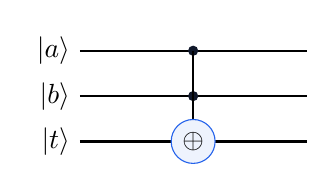
\begin{tikzpicture}[baseline=-0.55ex,scale=.72]
  \foreach \y/\n in {.8/a,0/b,-.8/t} {
    \draw[thick] (0,\y)--(4,\y);
    \node[left] at (0,\y) {$\ket{\n}$};
  }
  \fill[QpuNavy] (2,.8) circle (.09);
  \fill[QpuNavy] (2,0) circle (.09);
  \draw[thick] (2,.8)--(2,-.8);
  \node[draw=QpuBlue,fill=QpuBlue!8,circle,inner sep=2pt,font=\bfseries] at (2,-.8) {$\oplus$};
\end{tikzpicture}}

\newcommand{\SwapSegment}{%
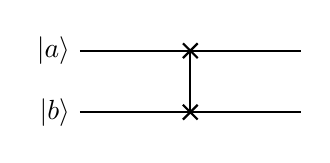
\begin{tikzpicture}[baseline=-0.55ex,scale=.78]
  \draw[thick] (0,.5)--(3.6,.5);
  \draw[thick] (0,-.5)--(3.6,-.5);
  \node[left] at (0,.5) {$\ket{a}$};
  \node[left] at (0,-.5) {$\ket{b}$};
  \draw[thick] (1.68,.38)--(1.92,.62) (1.68,.62)--(1.92,.38);
  \draw[thick] (1.68,-.38)--(1.92,-.62) (1.68,-.62)--(1.92,-.38);
  \draw[thick] (1.8,.5)--(1.8,-.5);
\end{tikzpicture}}

\newcommand{\QpuMeter}[2]{%
  \begin{scope}[shift={(#1,#2)}]
    \draw[QpuBlue,thick] (-0.28,-0.22) rectangle (0.28,0.28);
    \draw[QpuBlue,thick] (-0.18,-0.02) arc (180:0:0.18);
    \draw[QpuBlue,thick] (0,-0.02) -- (0.14,0.16);
    \fill[QpuBlue] (0,-0.02) circle (0.035);
  \end{scope}}
\newcommand{\MeasureSegment}{%
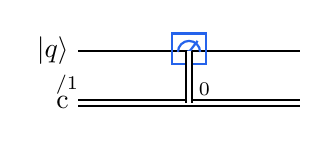
\begin{tikzpicture}[baseline=-0.55ex,scale=.78]
  \draw[thick] (0,0)--(3.6,0);
  \node[left] at (0,0) {$\ket{q}$};
  \QpuMeter{1.8}{0}
  \draw[double distance=1.4pt,thick] (0,-.85)--(3.6,-.85);
  \node[left] at (0,-.85) {c};
  \node[left,font=\scriptsize] at (0.15,-.55) {/1};
  \draw[double distance=1.4pt,thick] (1.8,0)--(1.8,-.85);
  \node[right,font=\scriptsize] at (1.8,-.62) {0};
\end{tikzpicture}}

% The hypertarget gives each gate a stable PDF named destination (gate-CNOT,
% gate-H, ...) that the workbench links to with #nameddest=.
\newcommand{\GateHeading}[3]{%
\subsection{#1 (\code{#2})}\hypertarget{gate-#2}{}
\begin{center}#3\end{center}}

% Short framed callouts. The body is boxed, so it cannot contain lstlisting
% and should stay short enough to fit on one page.
\newsavebox{\QpuCalloutBox}
\newenvironment{QpuCallout}[2]{%
  \def\QpuCalloutColor{#1}%
  \setlength{\fboxrule}{0.6pt}%
  \par\smallskip\noindent
  \begin{lrbox}{\QpuCalloutBox}%
  \begin{minipage}{\dimexpr\linewidth-2\fboxsep-2\fboxrule\relax}%
  \setlength{\parskip}{3pt}%
  {\bfseries\color{#1}#2}\par
}{%
  \end{minipage}%
  \end{lrbox}%
  \fcolorbox{\QpuCalloutColor}{\QpuCalloutColor!6}{\usebox{\QpuCalloutBox}}%
  \par\smallskip
}
\newenvironment{beginnerbox}[1][Beginner note]{\begin{QpuCallout}{QpuGreen}{#1}}{\end{QpuCallout}}
\newenvironment{trybox}[1][Try it in the Circuit builder]{\begin{QpuCallout}{QpuBlue}{#1}}{\end{QpuCallout}}
\newenvironment{cautionbox}[1][Watch out]{\begin{QpuCallout}{QpuAmber}{#1}}{\end{QpuCallout}}

% Workbench selectors on the left, the circuit diagram they produce on the
% right. #1 is the gate name shown in the Gate selector and on the target.
\newcommand{\WorkbenchControlMap}[1]{%
\begin{tikzpicture}[font=\small,>={Latex[length=2mm]}]
  \tikzset{ui/.style={draw=##1,rounded corners=2pt,anchor=west,minimum width=3.9cm,minimum height=.55cm,inner sep=3pt}}
  \node[ui=QpuLine,fill=CodeBg] at (0,1.75) {\textsf{Gate:} \textbf{#1}};
  \node[ui=QpuBlue,fill=QpuBlue!8] (a) at (0,.95) {\textsf{Control A:} \textbf{q0}};
  \node[ui=QpuBlue,fill=QpuBlue!8] (b) at (0,.15) {\textsf{Control B:} \textbf{q1}};
  \node[ui=QpuRed,fill=QpuRed!6] (t) at (0,-.65) {\textsf{Target particle:} \textbf{q2}};
  \node[font=\scriptsize\bfseries,color=QpuNavy,anchor=west] at (0,2.45) {Interactive workbench};
  \node[font=\scriptsize\bfseries,color=QpuNavy] at (7.4,2.45) {Circuit canvas};
  \foreach \y/\q in {.95/q0,.15/q1,-.65/q2} {
    \draw[thick] (5.6,\y)--(9.2,\y);
    \node[left,font=\scriptsize] at (5.6,\y) {\q};
  }
  \draw[->,dashed,QpuBlue] (a.east)--(5.05,.95);
  \draw[->,dashed,QpuBlue] (b.east)--(5.05,.15);
  \draw[->,dashed,QpuRed] (t.east)--(5.05,-.65);
  \fill[QpuNavy] (7.4,.95) circle (.09);
  \fill[QpuNavy] (7.4,.15) circle (.09);
  \draw[thick] (7.4,.95)--(7.4,-.65);
  \node[draw=QpuRed,fill=QpuRed!6,circle,inner sep=1.5pt,font=\bfseries] at (7.4,-.65) {$\oplus$};
  \node[anchor=west,font=\scriptsize] at (9.3,.95) {$A$: read, left unchanged};
  \node[anchor=west,font=\scriptsize] at (9.3,.15) {$B$: read, left unchanged};
  \node[anchor=west,font=\scriptsize] at (9.3,-.65) {$t' = t\oplus(A\land B)$: written};
\end{tikzpicture}}

\newcommand{\QpuTitlePage}{%
\begin{titlepage}
\pagecolor{QpuPaper}
\centering
\vspace*{1.15in}
{\Huge\bfseries\color{QpuNavy} \QpuDocTitle\par}
\vspace{0.2in}
{\LARGE\color{QpuBlue} \QpuDocSubtitle\par}
\vspace{0.55in}
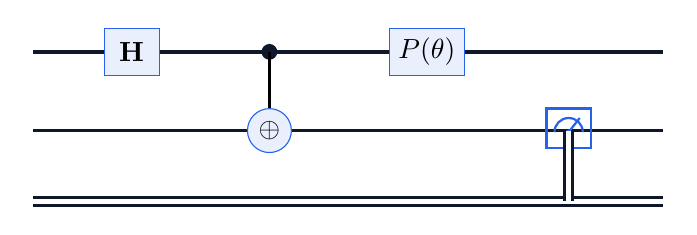
\begin{tikzpicture}
  \draw[very thick,QpuNavy] (0,1)--(8,1);
  \draw[very thick,QpuNavy] (0,0)--(8,0);
  \draw[double distance=1.6pt,very thick,QpuNavy] (0,-.9)--(8,-.9);
  \node[draw=QpuBlue,fill=QpuBlue!10,minimum width=.7cm,minimum height=.6cm,font=\bfseries] at (1.25,1) {H};
  \fill[QpuNavy] (3,1) circle (.1);
  \draw[very thick] (3,1)--(3,0);
  \node[draw=QpuBlue,fill=QpuBlue!10,circle,inner sep=2pt] at (3,0) {$\oplus$};
  \node[draw=QpuBlue,fill=QpuBlue!10,minimum width=.8cm,minimum height=.6cm,font=\bfseries] at (5,1) {$P(\theta)$};
  \QpuMeter{6.8}{0}
  \draw[double distance=1.6pt,very thick,QpuNavy] (6.8,0)--(6.8,-.9);
\end{tikzpicture}
\vfill
{\large Bailey Forbes\par}
{\large September 13, 2026\par}
\vspace{0.35in}
\begin{minipage}{0.82\textwidth}
\small\color{QpuNavy}
\QpuDocDescription
\end{minipage}
\vfill
\end{titlepage}
\nopagecolor
}

% Widen the TOC number column so two-digit subsections (13.10) keep a gap before the title.
\makeatletter
\renewcommand*\l@subsection{\@dottedtocline{2}{1.5em}{2.8em}}
\renewcommand*\l@subsubsection{\@dottedtocline{3}{4.3em}{3.6em}}
\makeatother

\newcommand{\QpuContents}{%
\pagenumbering{roman}
\tableofcontents
\clearpage
\pagenumbering{arabic}
}


\begin{document}
\QpuTitlePage
\QpuContents

\section{Scope and execution model}

The compiler turns a plain-text \code{.qpucir} protocol into one flat sequence
of circuit gates:
\[
\text{protocol source}\longrightarrow
\text{logical lines}\longrightarrow
\text{QPU instructions}\longrightarrow
\text{scoped tokens}\longrightarrow
\text{gates}\longrightarrow
\text{state-vector simulation}.
\]
Child processes are expanded at compile time. The UI and simulator therefore
see the same ordered gate list even when the source contains nested processes.

\subsection{Three levels of support}

\begin{tabularx}{\textwidth}{>{\bfseries}l X}
\toprule
Status & Meaning\\
\midrule
\implemented & The QPU language accepts the instruction and the compiler emits behavior
that the simulator executes.\\
\acceptedonly & The QPU language accepts the instruction and preserves it in compiler output or
the compiler log, but no visual/simulator operation is emitted yet.\\
\internal & The compiler may emit the operation itself, but protocol source
cannot name it directly. \code{RESET} is the important example.\\
\bottomrule
\end{tabularx}

\subsection{QPU instruction inventory}

\begin{longtable}{>{\ttfamily}p{0.24\textwidth}p{0.18\textwidth}p{0.48\textwidth}}
\toprule
\normalfont\bfseries Command & \bfseries Status & \bfseries Purpose\\
\midrule
\endhead
X, Y, Z, H, S, T, PHASE & \implemented & Single-qubit matrix operations.\\
CNOT, CCNOT, CZ, CY, SWAP & \implemented & Controlled and two-wire primitive operations.\\
NOT, AND, NAND, OR, XOR & \implemented & Derived logical target mutations.\\
MEASURE & \implemented & Measure one named wire or all known wires.\\
SET, CREATETOKEN & \implemented & Initialize/alias tokens and reserve wires.\\
RUNCHILD, CALL & \implemented & Expand a catalog/library child process.\\
RETURNVALS, ACCEPTVALS & \implemented & Bind child and process outputs.\\
MAIN-PROCESS, INCREASECYCLE & \implemented & Mark a process and flush cycle workspace.\\
DECLARECHILD & \implemented & Bind a catalog child for later RUNCHILD/CALL.\\
FREE, DELETETOKEN & \implemented & End a name. Reuse its wire only from a known $\ket0$.\\
JOIN, SPLIT & \implemented & Name an ordered register and a dimension-sized part of it.\\
COMPILEPROCESS & \implemented & Verify a child process without inlining its gates.\\
MASTERVAL & \implemented & Distinguished return. Does not add a truth-table column.\\
\code{SAVE_STATE}, \code{LOAD_STATE} & \implemented & Simulator checkpoints of the state vector and measurements.\\
\bottomrule
\end{longtable}

\textbf{Not source syntax:} \code{RESET} exists in the gate registry, but it is
not a supported source instruction. Write \code{SET wire 0p};
the compiler schedules internal \code{RESET} gates for zeroed workspace.


\section{Lexical and file syntax}

\subsection{Logical lines, whitespace, and case}

Commands and flags are case-insensitive and are separated by whitespace.
Token names retain their spelling. CRLF and LF line endings are accepted.
A physical line ending \emph{exactly} in a backslash joins to the next line:

\begin{lstlisting}
PARAMS: A:state B:state \
        Cin:state
CCNOT -I A B \
      -O Carry
\end{lstlisting}

The continuation backslash must be the final character; spaces after it prevent
continuation. Blank logical lines are discarded.

\subsection{Hash comments}

\begin{lstlisting}
# Whole-line or trailing hash comment
H -I Q:0 -O Q:0  # prepare |+>
\end{lstlisting}
A hash starts a comment that continues through the logical line. Comments are
for explanations and do not become instructions. Because continuation joining
happens first, a hash on a continued logical line can hide text that appeared
on a later physical line. Prefer comments after a complete instruction.

\subsection{Block comments}

\begin{lstlisting}
/* A block comment may span logical lines. */
PHASE=pi/2 -I Q:0 -O Q:0
\end{lstlisting}

Text from \code{/*} through \code{*/} is ignored. A block may occupy one line
or continue across several lines. Block comments are useful for temporarily
annotating a region, but they should not be nested. Keep delimiters visually
obvious so an omitted closing marker does not hide the remainder of a file.

\subsection{\code{PARAMS:}: the process input declaration}

\begin{lstlisting}
PARAMS: A:state B:state Theta:float Count:int
\end{lstlisting}

\code{PARAMS:} is recognized only when it is the first non-comment logical
line. Each whitespace-separated entry containing a colon becomes
\code{name:type}. Declaration order is interface order: RUNCHILD inputs and
truth-table input columns map from left to right.

Long declarations can use continuation:
\begin{lstlisting}
PARAMS: A0:state A1:state B0:state B1:state \
        Cin:state Width:int
\end{lstlisting}

The system retains the type text:
\begin{itemize}
  \item \code{state} entries become user-facing circuit inputs and truth-table
  input columns. Each participating state parameter resolves to a qubit wire.
  \item \code{int} and \code{float} entries are retained but excluded from
  user-facing qubit controls and truth-table state inputs. They describe
  numeric process metadata rather than prepared qubits.
  \item other type names are retained as written. Because they are not one of
  the recognized numeric exclusions, they may be exposed like stateful
  parameters; prefer \code{state}, \code{int}, or \code{float} for predictable
  behavior.
\end{itemize}

PARAMS has a colon after the keyword; \code{MAIN-PROCESS} does not. An empty or
misplaced PARAMS line is not a substitute for a valid first-line declaration.
The process's MAIN-PROCESS instruction is described in the composition chapter.

\subsection{Protocol file forms}

The normal authoring format is plain UTF-8 QPU text saved as
\code{ProcessName.qpucir}. A \code{.qpucir.txt} download is also plain source
and is useful where browsers or editors insist on a text extension. Uploading
plain text derives the display name from MAIN-PROCESS.

The loader can also accept a JSON export envelope:
\begin{lstlisting}[language={}]
{
  "format": "qpucir",
  "version": 1,
  "name": "First circuit",
  "source": "MAIN-PROCESS FirstCircuit\nRETURNVALS Q"
}
\end{lstlisting}
The source string is the authoritative language text. Export envelopes may
also contain compiled qubit count, gates, token map, and export timestamp
metadata, but compilation from source determines current behavior.


\section{Names and token references}

A \emph{token} is the QPU language's name for a logical storage location. For
the circuits in this guide, a token normally identifies one qubit wire.
Instructions refer to tokens instead of physical machine addresses. During
compilation, the system resolves each live token to an integer qubit index.
This indirection makes protocols readable and lets child processes have private
workspace without colliding with their parents.

\subsection{Token names}

A bare token is written as a whitespace-delimited name:
\begin{lstlisting}
Q
Control
CarryOut
scratch_2
0
\end{lstlisting}
Names are case-sensitive even though instruction names are not:
\code{Carry} and \code{carry} are distinct tokens. A name cannot contain
whitespace because whitespace separates language elements. Avoid names that
begin with a hyphen: inside a flag list, any hyphen-prefixed token is treated
as the beginning of another flag.

Tokens are allocated lazily. Mentioning a token in a gate, a state-setting
instruction, or \code{CREATETOKEN} gives it a wire when compilation needs one.
Consequently, source order affects the internal numeric wire index, but not the
meaning of a consistently named circuit.

\subsection{Direct references}

A direct reference is simply the token's name:
\begin{lstlisting}
SET Q 0p
H -I Q -O Q
MEASURE -I Q
RETURNVALS Q
\end{lstlisting}
Every occurrence resolves to the same token within that process invocation.
For a one-qubit gate, repeat the name after both \code{-I} and \code{-O}.
This does not copy the state. It says that Q is the instruction's incoming
wire and that the same Q wire is mutated in place.

\subsection{Parameter references with a dollar sign}

A leading dollar sign is the explicit parameter/reference spelling:
\begin{lstlisting}
PARAMS: Input:state
MAIN-PROCESS DollarReference
SET Local $Input
H -I $Input -O $Input
RETURNVALS Local
\end{lstlisting}
Address resolution removes the leading \code{$}. Thus \code{Input} and
\code{$Input} ultimately refer to the same declared parameter. The dollar
form is especially useful inside reusable child protocols because it visually
separates caller-supplied values from child-local workspace.

\code{SET Local \$Input} creates an alias: Local resolves to the same underlying
wire as Input. It does \emph{not} clone an unknown quantum state. Quantum states
cannot generally be copied because of the no-cloning theorem; aliasing avoids
claiming that a physical copy occurred.

\subsection{Cycle-qualified references with \code{:}}

A token may carry a suffix after a colon:
\begin{lstlisting}
Q:0
Q:1
Carry:next
\end{lstlisting}
The current system strips the colon and everything after it when mapping source
references to visual qubit wires. Therefore all three examples above whose
base is Q---\code{Q:0}, \code{Q:1}, and bare \code{Q}---identify the same
logical wire. The suffix is protocol notation for a stage, cycle, or bit
version; it does not create a second qubit.

\begin{lstlisting}
SET Q:0 0p
H -I Q:0 -O Q:1
MEASURE -I Q:2
\end{lstlisting}
This example applies H to one wire and then measures that same wire. The
changing suffix communicates progression to a human reader, while
\code{INCREASECYCLE} provides the actual compiler cycle boundary.

\textbf{Practical rule:} if two values must exist simultaneously, give them
different base names. Do not expect \code{Q:0} and \code{Q:1} to hold two
independent states.

\subsection{Aliases created by \code{SET}}

When the second operand of SET is not a built-in state constant, SET creates a
name alias:
\begin{lstlisting}
SET Working Input
SET Output Working
X -I Output -O Output
\end{lstlisting}
After resolution, Working, Output, and Input name one wire. Mutating any alias
mutates that wire for every alias. This behavior is useful for readable names
and process binding, but it is not assignment in the classical
``copy a value into a new variable'' sense.

Aliases are resolved within a process frame. PARAMS and parent/child bindings
take precedence over ordinary child-local scoping, ensuring that an operation
on a bound parameter affects the caller's intended wire.

\subsection{Numeric workspace references}

Bare numeric names such as \code{0}, \code{1}, and \code{2} are valid token
names and are common in reusable arithmetic children:
\begin{lstlisting}
SET 0:0 $A
SET 1:0 $B
SET 2:0 $Cin
\end{lstlisting}
When a child process uses a numeric workspace name, the compiler places it in
the parent invocation's workspace namespace. This lets nested adders reuse the
same compact source names without globally identifying every child invocation's
scratch wires.

Numeric token names are not number literals. \code{2} names a wire; it does not
mean the integer two or the basis state $\ket{2}$.

\subsection{Process scope and child-local references}

Each process invocation receives a unique scope. A local name such as
\code{Scratch} in two separate child calls therefore denotes two separately
resolved local references unless output or parameter binding deliberately joins
them. Conceptually, compilation turns:
\begin{lstlisting}
RUNCHILD Worker -I A -O First
RUNCHILD Worker -I B -O Second
\end{lstlisting}
into two independent Worker frames. This is similar to local variables in two
function calls. PARAMS map caller references into the frame, and RETURNVALS map
selected frame references back out.


\section{Built-in state constants}

State constants describe how a wire begins. They are not ordinary token names,
even though they participate in address resolution. Constants are
case-insensitive and may be written with a leading dollar sign. The three
supported base constants are \code{0p}, \code{1p}, and \code{sp}; the letter
\code{p} distinguishes protocol state notation from ordinary numbers.

\subsection{\code{0p}: the zero basis state}

\code{0p} denotes
\[
\ket0=\begin{bmatrix}1\\0\end{bmatrix}.
\]
\begin{lstlisting}
SET Output 0p
\end{lstlisting}
For workspace, this schedules zero preparation. The compiler batches pending
zero preparations into internal RESET operations immediately before the next
real gate, at an \code{INCREASECYCLE}, or at process end. RESET is deliberately
not source syntax; \code{SET Output 0p} is the public way to request zero.

Zero is the usual target initialization for reversible AND, OR, and XOR:
with $t=0$, the mutation $t\leftarrow t\oplus f(x)$ leaves $t=f(x)$.

\subsection{\code{1p}: the one basis state}

\code{1p} denotes
\[
\ket1=\begin{bmatrix}0\\1\end{bmatrix}.
\]
\begin{lstlisting}
SET Flag 1p
\end{lstlisting}
The compiler realizes one preparation by applying X to a zero-initialized
wire. A target beginning in one is useful when the desired reversible result is
the complement of a Boolean predicate. For example,
$1\oplus(A\land B)=\neg(A\land B)$, which is NAND.

\subsection{\code{sp}: equal superposition}

\code{sp} denotes the plus state
\[
\ket+=\frac{\ket0+\ket1}{\sqrt2}
=\frac1{\sqrt2}\begin{bmatrix}1\\1\end{bmatrix}.
\]
\begin{lstlisting}
SET Probe sp
\end{lstlisting}
The compiler realizes this preparation with a Hadamard gate. If immediately
measured, the result is 0 or 1 with equal probability. It is not merely a hidden
classical random bit: both amplitudes coexist and can interfere after later
phase and Hadamard operations.

In an expected truth-table \emph{output} cell, \code{sp} has a different
testing role: it means either measured bit is acceptable. Context therefore
matters---protocol SET initializes a plus state, while expected output metadata
uses \code{sp} as a don't-care marker.

\subsection{Dimension-suffixed constants}

The language also recognizes:
\begin{lstlisting}
0p_dim2
1p_dim8
sp_dim4
\end{lstlisting}
The suffix must be \code{_dim} followed by a power of two that is at least 2.
That number is a Hilbert-space dimension, so \code{_dim4} prepares two qubits
and \code{_dim8} prepares three. \code{0p} prepares every wire in $\ket0$,
\code{1p} flips only the least-significant wire, and \code{sp} applies H to
every wire. \code{_dim2} is the same one-wire preparation as the unsuffixed
constant. Any other dimension is rejected. Wire $k$ of register \code{R} is
named \code{R[k]}.

\subsection{Constants and state parameters}

For an ordinary local token, SET emits preparation behavior. For a PARAMS entry
typed \code{state}, SET supplies a default instead:
\begin{lstlisting}
PARAMS: Input:state
MAIN-PROCESS DefaultInput
SET Input 0p
X -I Input -O Input
RETURNVALS Input
\end{lstlisting}
The UI or truth-table runner may replace the default start state for Input.
This distinction is what allows one compiled protocol to be tested over every
binary input row instead of hard-wiring its parameter to zero.


\section{Instruction flags and argument boundaries}

\subsection{\code{-I}: input and control references}

\code{-I} begins the instruction's input list:
\begin{lstlisting}
H     -I Target       -O Target
CNOT -I Control      -O Target
CCNOT -I A B          -O Target
\end{lstlisting}
Its interpretation depends on the gate. For a one-qubit gate, the input names
the same wire that the output mutates. For CNOT/CZ/CY it names one control. For
CCNOT and the two-input derived logic gates it names two controls. Input order
does not matter to symmetric predicates such as AND or XOR, but it remains part
of the written instruction and should be kept consistent for readability.

\subsection{\code{-O}: output and target references}

\code{-O} begins the output list. For most gates its first token is the target
wire whose amplitudes are changed:
\begin{lstlisting}
X -I Q -O Q
AND -I A B -O Result
\end{lstlisting}
\code{-O} does not mean ``allocate a fresh classical output.'' The target may
already contain a quantum state, and reversible logic XORs its result into that
existing state. SWAP is exceptional: it requires two outputs matching its two
inputs. MEASURE takes no output flag because the measurement map stores its
classical result.

\subsection{\code{-IF}: classical feed-forward (optional)}

A gate may carry a forward-only classical condition after a prior MEASURE:
\begin{lstlisting}
X -I Bob -O Bob -IF Alice=1
Z -I Bob -O Bob -IF M0=1
\end{lstlisting}
The named token must already have been measured; running a conditioned gate
before its MEASURE is a runtime error. If the classical bit does not match,
the gate is skipped and execution continues. The skipped gate stays in the
circuit. To condition several gates, or to pair a gate with an alternative,
use the structured \code{IF} / \code{ELSE} / \code{ENDIF} block described in
\hyperlink{if-else-blocks}{Structured classical branches}; it lowers to the
same \code{-IF} conditions. Either way there is no backward edge---the circuit
remains a finite ordered list.

\subsection{Where a flag list ends}

An \code{-I} or \code{-O} list continues until the next token beginning with a
hyphen or the end of the line:
\begin{lstlisting}
CCNOT -I A B -O Carry -$R
\end{lstlisting}
Here A and B belong to \code{-I}, Carry belongs to \code{-O}, and
\code{-$R} starts a separate flag. This rule is why token names should not
begin with a hyphen.

Flags are case-insensitive, so \code{-i} and \code{-o} work, but uppercase is
the documented style. Supplying flags in an unusual order may still parse, but
\code{-I} followed by \code{-O} is the clearest and matches generated source.

\subsection{No-parameter-substitution marker}

\begin{lstlisting}
PHASE=pi/4 -I Q -O Q -$R
\end{lstlisting}
The language recognizes this marker and, on that instruction only, resolves
names as locals instead of substituting \code{PARAMS} bindings. Aliases created
by \code{SET} still apply.

\subsection{Positional arguments}

Not every instruction uses flags. SET, MAIN-PROCESS, RETURNVALS, ACCEPTVALS,
and several compatibility instructions consume positional words:
\begin{lstlisting}
SET Target 0p
MAIN-PROCESS Example
RETURNVALS Carry Sum
\end{lstlisting}
The command name is the first word and positional arguments follow in order.
RETURNVALS order is part of the process interface. For non-gate compatibility
instructions, extra words may be retained even when no execution behavior is
defined; accepted text should not be mistaken for an implemented effect.


\section{Gate instruction grammar and arity}

\subsection{General gate shape}

\begin{lstlisting}
GATE -I input_or_controls -O target
\end{lstlisting}
The uppercase word selects a gate. \code{-I} lists the incoming wire for a
one-qubit operation or the controls for a controlled operation. \code{-O}
names the wire that is mutated. Except for SWAP, gate instructions do not
create a separate output wire automatically.

\begin{lstlisting}
H -I Q -O Q
CNOT -I Control -O Target
\end{lstlisting}
In the first row, Q is listed twice because the state flows through H on one
wire. In the second, Control is preserved and Target is conditionally changed.

\subsection{Why arity matters}

\begin{center}
\begin{tabular}{lll}
\toprule
Gate family & Required \code{-I} count & Required \code{-O} count\\
\midrule
X, Y, Z, H, S, T, PHASE, NOT & 1 & 1\\
CNOT, CZ, CY & 1 & 1\\
CCNOT, AND, NAND, OR, XOR & 2 & 1\\
SWAP & 2 & 2\\
MEASURE & 0 or 1 & 0\\
\bottomrule
\end{tabular}
\end{center}

All counts are exact except \code{MEASURE}. For ordinary single-qubit gates,
name the same wire in \code{-I} and \code{-O}. The output is the mutated target;
for controlled gates, \code{-I} contains controls.

\subsection{Validation and common mistakes}

Arity is part of the language contract. A CNOT with two inputs is not silently
converted into CCNOT, and a CCNOT with one input is not converted into CNOT.
The compiler reports whether an instruction has too few or too many inputs or
outputs.

\begin{lstlisting}
# Wrong: H needs one output.
H -I Q

# Wrong: CNOT needs exactly one control.
CNOT -I A B -O Target

# Right:
CCNOT -I A B -O Target
\end{lstlisting}

The target is removed from the compiler's control list if the same resolved
wire appears on both sides. This is necessary for the normal one-qubit form.
For controlled gates, do not also list the target as an input; doing so either
violates arity or obscures the intended control relationship.


\section{Single-qubit primitive gates}

\GateHeading{Pauli X}{X}{\GateSegment{X}}

\[
X=\begin{bmatrix}0&1\\1&0\end{bmatrix},\quad
X\ket0=\ket1,\quad X\ket1=\ket0,\quad
X(\alpha\ket0+\beta\ket1)=\beta\ket0+\alpha\ket1.
\]
X is the quantum bit flip. On the Bloch sphere it is a half-turn around the
x-axis. It exchanges the north and south poles and is self-inverse:
$X^2=I$. Unlike a classical NOT implementation, X remains meaningful on a
superposition because it exchanges amplitudes linearly without measuring.
\begin{lstlisting}
X -I Q:0 -O Q:0
\end{lstlisting}
\begin{center}
\begin{tabular}{ccc}\toprule Input & Classical comparison & Output\\\midrule
0 & NOT 0 & 1\\
1 & NOT 1 & 0\\\bottomrule\end{tabular}
\end{center}

\GateHeading{Pauli Y}{Y}{\GateSegment{Y}}

\[
Y=\begin{bmatrix}0&-i\\i&0\end{bmatrix},\quad
Y\ket0=i\ket1,\quad Y\ket1=-i\ket0.
\]
It flips the basis value like X but adds phases that become observable through
later interference. Geometrically it is a half-turn around the y-axis and is
self-inverse, $Y^2=I$. The factors $i$ and $-i$ are global phases for either
basis state by itself, but on components of a larger superposition they may
become relative phases.
\begin{lstlisting}
Y -I Q -O Q
\end{lstlisting}
\begin{center}
\begin{tabular}{ccc}\toprule Input & Measured bit & Quantum output\\\midrule
0 & 1 & $i\ket1$\\
1 & 0 & $-i\ket0$\\\bottomrule\end{tabular}
\end{center}

\GateHeading{Pauli Z}{Z}{\GateSegment{Z}}

\[
Z=\begin{bmatrix}1&0\\0&-1\end{bmatrix},\quad
Z\ket0=\ket0,\quad Z\ket1=-\ket1.
\]
Z does not change a computational-basis measurement, but it changes relative
phase. For example, $Z\ket+=\ket-=(\ket0-\ket1)/\sqrt2$.
On the Bloch sphere it is a half-turn around z. It is self-inverse and is the
simplest example showing why quantum state cannot be reduced to a table of
immediate measurement probabilities.
\begin{lstlisting}
Z -I Q -O Q
\end{lstlisting}
\begin{center}
\begin{tabular}{ccc}\toprule Input & Classical bit & Quantum output\\\midrule
0 & 0 & $\ket0$\\
1 & 1 & $-\ket1$\\\bottomrule\end{tabular}
\end{center}

\GateHeading{Hadamard}{H}{\GateSegment{H}}

\[
H=\frac1{\sqrt2}\begin{bmatrix}1&1\\1&-1\end{bmatrix},\quad
H\ket0=\ket+,\quad H\ket1=\ket-.
\]
Hadamard changes between the computational z basis and the plus/minus x basis.
It creates equal magnitudes from a basis state, but the sign of the second
amplitude depends on the input. It is also self-inverse: applying H twice
returns the original state. H is commonly used before controlled gates to
create entanglement and after phase gates to reveal interference.
\begin{lstlisting}
SET Q 0p
H -I Q -O Q
MEASURE -I Q
\end{lstlisting}
\begin{center}
\begin{tabular}{ccc}\toprule Input & Measurement distribution & State before measurement\\\midrule
0 & 50\% 0, 50\% 1 & $(\ket0+\ket1)/\sqrt2$\\
1 & 50\% 0, 50\% 1 & $(\ket0-\ket1)/\sqrt2$\\\bottomrule\end{tabular}
\end{center}
Equal classical probabilities hide the relative minus sign responsible for
interference.

\GateHeading{S phase}{S}{\GateSegment{S}}

\[
S=P(\pi/2)=\begin{bmatrix}1&0\\0&i\end{bmatrix},\qquad
S\ket1=i\ket1,\qquad S^2=Z.
\]
S is a quarter-turn around the Bloch sphere's z-axis. It changes $\ket+$ into
$(\ket0+i\ket1)/\sqrt2$ while leaving basis measurement probabilities
unchanged. Its inverse is $S^\dagger=P(-\pi/2)$, not S itself.
\begin{lstlisting}
S -I Q -O Q
\end{lstlisting}
\begin{center}
\begin{tabular}{ccc}\toprule Input & Measured bit & Quantum output\\\midrule
0 & 0 & $\ket0$\\
1 & 1 & $i\ket1$\\\bottomrule\end{tabular}
\end{center}

\GateHeading{T phase}{T}{\GateSegment{T}}

\[
T=P(\pi/4)=\begin{bmatrix}1&0\\0&e^{i\pi/4}\end{bmatrix},\qquad
T^2=S,\qquad T^4=Z.
\]
T is an eighth-turn around z. Together with gates such as H and CNOT, it is an
important non-Clifford resource for expressing general quantum computations.
Its inverse is $T^\dagger=P(-\pi/4)$; the current \code{BT} spelling does not
synthesize that inverse, so use \code{BPHASE=pi/4} when the negative phase is
required.
\begin{lstlisting}
T -I Q -O Q
\end{lstlisting}
\begin{center}
\begin{tabular}{ccc}\toprule Input & Measured bit & Quantum output\\\midrule
0 & 0 & $\ket0$\\
1 & 1 & $e^{i\pi/4}\ket1$\\\bottomrule\end{tabular}
\end{center}

\GateHeading{Arbitrary phase}{PHASE}{\GateSegment{$P(\theta)$}}

\[
P(\theta)=\begin{bmatrix}1&0\\0&e^{i\theta}\end{bmatrix},\qquad
\alpha\ket0+\beta\ket1\mapsto
\alpha\ket0+\beta e^{i\theta}\ket1.
\]
PHASE is the general form behind S, T, and Z. It preserves
$|\alpha|^2$ and $|\beta|^2$ because $|e^{i\theta}|=1$, yet rotates the
relative phase by $\theta$. On the Bloch sphere this is a z-axis rotation up to
global phase. A later H or another basis-changing gate is normally needed to
turn that phase difference into changed computational-basis probabilities.
The angle is embedded in the opcode:
\begin{lstlisting}
PHASE=1.5708 -I Q -O Q     # radians
PHASE=3/2 -I Q -O Q        # rational radians
PHASE=90d -I Q -O Q        # degrees
PHASE=45/2d -I Q -O Q      # rational degrees
PHASE=pi -I Q -O Q
PHASE=-11pi/6 -I Q -O Q
PHASE=2*pi/3 -I Q -O Q
BPHASE=pi/4 -I Q -O Q      # P(-pi/4)
\end{lstlisting}
Accepted numeric atoms include signed integers, decimals, leading-dot decimals,
and one optional rational denominator. Pi notation accepts an optional sign,
an integer coefficient, an optional \code{*}, and an optional positive integer
denominator. A zero denominator and malformed angle raise an error.

\begin{center}
\begin{tabular}{ccc}\toprule Input & Measured bit & Quantum output\\\midrule
0 & 0 & $\ket0$\\
1 & 1 & $e^{i\theta}\ket1$\\\bottomrule\end{tabular}
\end{center}

\subsection{Backward-prefix syntax}

The QPU language recognizes a leading \code{B} before a supported primitive gate name,
for example \code{BX}, \code{BH}, \code{BCNOT}, or \code{BSWAP}, and sets
\code{reverse=true}. (Compiler-internal \code{RESET} remains unavailable in
source.) Only \code{BPHASE=angle} currently changes emitted behavior: the
compiler negates the phase angle. For every other gate the flag is metadata
only. Emitting the ordinary gate still gives the mathematical inverse for these
self-inverse gates:
\[
X,\ Y,\ Z,\ H,\ \mathrm{CNOT},\ \mathrm{CCNOT},\
\mathrm{CZ},\ \mathrm{CY},\ \mathrm{SWAP}.
\]
In contrast, \code{BS} and \code{BT} do not synthesize $S^\dagger$ or
$T^\dagger$. Do not rely on B-prefixed forms for inverse execution unless the
gate is self-inverse or is \code{BPHASE}.


\section{Controlled and two-qubit primitive gates}

\GateHeading{Controlled NOT}{CNOT}{\ControlledSegment{$\oplus$}}

\[
\ket{c,t}\longmapsto\ket{c,t\oplus c}.
\]
CNOT leaves the control unchanged. When the control is zero, the target is
unchanged; when the control is one, X acts on the target. Because the map is a
permutation of basis states, it is reversible and self-inverse. A
superposition control can entangle the wires, so ``classical XOR'' describes
only its basis-state action.
\begin{lstlisting}
CNOT -I Control -O Target
\end{lstlisting}
\begin{center}
\begin{tabular}{cc|cc}\toprule $c$&$t$&$c'$&$t'$\\\midrule
0&0&0&0\\0&1&0&1\\1&0&1&1\\1&1&1&0\\\bottomrule
\end{tabular}
\end{center}
CNOT is a reversible embedding of XOR because it preserves the control.
In the workbench, the control comes from \textbf{Control A} and the target
from \textbf{Target particle}; \textbf{Control B} is ignored.

\GateHeading{Doubly controlled NOT / Toffoli}{CCNOT}{\DoubleControlledSegment}

\[
\ket{a,b,t}\longmapsto\ket{a,b,t\oplus(a\land b)}.
\]
CCNOT, also called Toffoli, applies X only when both controls are one. It is a
reversible universal building block for classical computation embedded in a
quantum circuit. The target's previous value matters: zero computes AND, while
one computes NAND. The gate is self-inverse.
\begin{lstlisting}
CCNOT -I A B -O Target
\end{lstlisting}
\begin{center}
\begin{tabular}{ccc|ccc}\toprule $a$&$b$&$t$&$a'$&$b'$&$t'$\\\midrule
0&0&0&0&0&0\\0&0&1&0&0&1\\
0&1&0&0&1&0\\0&1&1&0&1&1\\
1&0&0&1&0&0\\1&0&1&1&0&1\\
1&1&0&1&1&1\\1&1&1&1&1&0\\\bottomrule
\end{tabular}
\end{center}
With a target initialized to zero, Toffoli computes classical AND reversibly.

\begin{beginnerbox}[Controls are preserved, the target is the output]
In the table, the $a'$ and $b'$ columns always equal $a$ and $b$: the two
controls are only read. Only $t$ can change, and it flips exactly in the two
rows where $a=b=1$. In the \textbf{Interactive workbench}, choose
\textbf{CCNOT} in \textbf{Gate}, the two inputs in \textbf{Control A} and
\textbf{Control B}, and the output wire in \textbf{Target particle}. The
\emph{CCNOT demo} starter circuit is exactly this gate with both controls
prepared as 1.
\end{beginnerbox}

\GateHeading{Controlled Z}{CZ}{\ControlledSegment{Z}}

\[
\mathrm{CZ}\ket{c,t}=(-1)^{ct}\ket{c,t},\qquad
\mathrm{CZ}=\operatorname{diag}(1,1,1,-1).
\]
CZ adds a minus sign only to the $\ket{11}$ amplitude. No computational-basis
bit changes, but superpositions can acquire observable relative phase. CZ is
symmetric between its two wires, even though QPU syntax writes one as the
input control and one as the output target. It is self-inverse.
\begin{lstlisting}
CZ -I Control -O Target
\end{lstlisting}
\begin{center}
\begin{tabular}{cc|cc}\toprule Input & Measured output & Amplitude multiplier & State\\\midrule
00&00&$+1$&$\ket{00}$\\01&01&$+1$&$\ket{01}$\\
10&10&$+1$&$\ket{10}$\\11&11&$-1$&$-\ket{11}$\\\bottomrule
\end{tabular}
\end{center}
The classical columns are unchanged; the quantum phase is the operation.

\GateHeading{Controlled phase}{CPHASE}{\ControlledSegment{$P(\theta)$}}

\[
\ket{11}\longmapsto e^{i\theta}\ket{11},
\]
while $\ket{00}$, $\ket{01}$, and $\ket{10}$ are unchanged. CZ is the special
case $\theta=\pi$. CPHASE unlocks compact Quantum Fourier Transform and
phase-estimation demos.
\begin{lstlisting}
CPHASE=pi/2 -I Control -O Target
CPHASE=90d -I Control -O Target
\end{lstlisting}

\GateHeading{Controlled Y}{CY}{\ControlledSegment{Y}}

\[
\ket{0,t}\mapsto\ket{0,t},\quad
\ket{1,0}\mapsto i\ket{1,1},\quad
\ket{1,1}\mapsto-i\ket{1,0}.
\]
CY applies the Pauli Y rotation to the target only when the control is one. Its
basis-bit pattern resembles CNOT, but the $\pm i$ factors distinguish their
behavior on superpositions. Since $Y^2=I$, CY is self-inverse.
\begin{lstlisting}
CY -I Control -O Target
\end{lstlisting}
\begin{center}
\begin{tabular}{cc|cc|c}\toprule $c$&$t$&$c'$&$t'$&Quantum phase\\\midrule
0&0&0&0&$+1$\\0&1&0&1&$+1$\\
1&0&1&1&$i$\\1&1&1&0&$-i$\\\bottomrule
\end{tabular}
\end{center}

\GateHeading{Swap}{SWAP}{\SwapSegment}

\[
\mathrm{SWAP}\ket{a,b}=\ket{b,a}.
\]
SWAP exchanges the complete quantum states of two wires, including amplitudes
and any correlations with the rest of the register. It does not copy either
state. Three CNOTs can decompose SWAP, but the QPU system provides it as one
primitive instruction. Applying SWAP twice restores the original ordering.
\begin{lstlisting}
SWAP -I A B -O A B
\end{lstlisting}
The two output tokens are mandatory and must resolve to the same two wires, in
the same order, as the inputs.
\begin{center}
\begin{tabular}{cc|cc}\toprule $a$&$b$&$a'$&$b'$\\\midrule
0&0&0&0\\0&1&1&0\\1&0&0&1\\1&1&1&1\\\bottomrule
\end{tabular}
\end{center}


\section{Derived logical gates}

Derived gates are QPU instructions implemented as reversible target
mutations. Inputs are preserved. If target $t$ starts in zero, AND/OR/XOR
write the familiar classical function. If it does not, the true behavior is
the XOR embedding shown below.

\begin{beginnerbox}[One shape for every two-input gate]
AND, NAND, OR, and XOR all follow $t' = t\oplus f(a,b)$. The two inputs $a$
and $b$ (\textbf{Control A} and \textbf{Control B} in the workbench) are read
and left unchanged. The target $t$ (\textbf{Target particle}) is the output
workspace and is the only wire that changes. Only $f$ differs between the
four gates. To get the ordinary classical answer, start the target at 0 with
\code{SET Out 0p}.
\end{beginnerbox}

\GateHeading{Logical NOT}{NOT}{\GateSegment{$\neg$}}

\[
t'\;=\;t\oplus1.
\]
NOT is the derived logical spelling of a bit flip. In the current simulator it
uses the same X matrix on the output target. The required input establishes the
one-input instruction shape, but a distinct input is not copied into the
output; use the same token on both sides.
\begin{lstlisting}
NOT -I Target -O Target
\end{lstlisting}
\begin{center}
\begin{tabular}{c|c}\toprule $t$&$t'$\\\midrule0&1\\1&0\\\bottomrule\end{tabular}
\end{center}
The current gate implementation mutates the output target. Use the same token
for input and output; a distinct input token is not copied.

\GateHeading{Reversible AND}{AND}{\DoubleControlledSegment}

\[
t'=t\oplus(a\land b).
\]
AND flips the target exactly on the basis components where both controls are
one. This is Toffoli-style behavior. It remains linear on superpositions and
may entangle the target with its controls. Calling it AND is convenient only
when the target is deliberately initialized.
\begin{lstlisting}
SET Out 0p
AND -I A B -O Out
\end{lstlisting}
\begin{center}
\begin{tabular}{cc|c|c}\toprule $a$&$b$&$t=0$&$t'=a\land b$\\\midrule
0&0&0&0\\0&1&0&0\\1&0&0&0\\1&1&0&1\\\bottomrule
\end{tabular}
\end{center}

\GateHeading{Reversible NAND}{NAND}{\DoubleControlledSegment}

\[
t'=t\oplus(a\land b)\oplus1.
\]
NAND first performs the all-controls-active mutation and then inverts the
target. With target zero it produces the familiar NAND column. With target one
it instead produces AND, illustrating why reversible target state must always
be included in the full mathematical definition.
\begin{lstlisting}
SET Out 0p
NAND -I A B -O Out
\end{lstlisting}
\begin{center}
\begin{tabular}{cc|c|c}\toprule $a$&$b$&$t=0$&$t'=\neg(a\land b)$\\\midrule
0&0&0&1\\0&1&0&1\\1&0&0&1\\1&1&0&0\\\bottomrule
\end{tabular}
\end{center}

\GateHeading{Reversible OR}{OR}{\DoubleControlledSegment}

\[
t'=t\oplus(a\lor b).
\]
OR uses an ``any control is one'' predicate. If either or both controls are
active, the target is flipped. This direct derived operation is equivalent on
basis states to combining XOR and AND through
$a\lor b=a\oplus b\oplus(a\land b)$.
\begin{lstlisting}
SET Out 0p
OR -I A B -O Out
\end{lstlisting}
\begin{center}
\begin{tabular}{cc|c|c}\toprule $a$&$b$&$t=0$&$t'=a\lor b$\\\midrule
0&0&0&0\\0&1&0&1\\1&0&0&1\\1&1&0&1\\\bottomrule
\end{tabular}
\end{center}
For bits, $a\lor b=a\oplus b\oplus(a\land b)$.

\GateHeading{Reversible XOR}{XOR}{\DoubleControlledSegment}

\[
t'=t\oplus a\oplus b.
\]
XOR flips the target when an odd number of controls is one. With two inputs,
this is the ordinary exclusive-or predicate. The parity definition explains
why the 11 row does not flip: two active controls have even parity.
\begin{lstlisting}
SET Out 0p
XOR -I A B -O Out
\end{lstlisting}
\begin{center}
\begin{tabular}{cc|c|c}\toprule $a$&$b$&$t=0$&$t'=a\oplus b$\\\midrule
0&0&0&0\\0&1&0&1\\1&0&0&1\\1&1&0&0\\\bottomrule
\end{tabular}
\end{center}


\section{Measurement gate}

\GateHeading{Measurement}{MEASURE}{\MeasureSegment}

\begin{lstlisting}
MEASURE -I Q     # exactly one named wire
MEASURE          # every wire known at this point
\end{lstlisting}
\code{MEASURE} takes no \code{-O}. Repeated one-wire commands are useful when
only declared returns should become classical. A bare command emits one
measurement operation per currently allocated wire.

\begin{center}
\begin{tabular}{c|c|c}\toprule State & Outcome probabilities & Collapsed state\\\midrule
$\ket0$ & $P(0)=1$ & $\ket0$\\
$\ket1$ & $P(1)=1$ & $\ket1$\\
$\alpha\ket0+\beta\ket1$ & $P(0)=|\alpha|^2$, $P(1)=|\beta|^2$ &
$\ket0$ or $\ket1$\\\bottomrule
\end{tabular}
\end{center}


\section{State, token, and cycle commands}

\subsection{\code{SET} --- initialize or alias (\implemented)}

\begin{lstlisting}
SET Q 0p
SET Q 1p
SET Q sp
SET Local $Parameter
\end{lstlisting}
\code{SET target value} requires a positional value. A constant schedules or
emits initialization: zero, X from zero, or H from zero. A nonconstant value
makes the target an alias of that source. A \code{state} parameter's constant
SET is treated as a runtime default, allowing the UI or truth-table runner to
supply its actual start state.

\textbf{Syntax:} exactly one target and one value are meaningful. SET has no
\code{-I} or \code{-O} flags. It does not perform classical assignment at each
simulation step; it establishes compilation-time preparation or reference
identity. See the dedicated constants and aliases chapters before using SET on
unknown quantum data.

\subsection{\code{CREATETOKEN} --- reserve wires (\implemented)}

\begin{lstlisting}
CREATETOKEN -I Sum Carry Workspace
\end{lstlisting}
Every \code{-I} token immediately claims a stable wire index. No \code{-O} is
used. This is useful for declared outputs before their first gate.

\code{CREATETOKEN} does not initialize amplitudes by itself. Pair new workspace
with SET before relying on its value. Listing outputs early also makes process
structure easier to review:
\begin{lstlisting}
CREATETOKEN -I Sum Carry
SET Sum 0p
SET Carry 0p
\end{lstlisting}

\subsection{\code{DELETETOKEN} --- end a token name (\implemented)}

\begin{lstlisting}
DELETETOKEN -I Workspace
\end{lstlisting}
The named token leaves scope. A later use is a compile error. The wire is
returned to the allocator only when it is already known to be $\ket0$, which
is the state after \code{SET wire 0p} and before any gate targets it. Deletion
does not emit \code{RESET} and does not erase an unknown or entangled state.

\subsection{\code{FREE} --- same lifetime rule (\implemented)}

\begin{lstlisting}
FREE -I ScratchA ScratchB
\end{lstlisting}
FREE uses the same rule as DELETETOKEN. Use \code{SET wire 0p} when the
intended behavior is zero preparation. A wire that is not known $\ket0$ keeps
its qubit index, and only the name dies.

\subsection{\code{INCREASECYCLE} --- cycle boundary (\implemented)}

\begin{lstlisting}
INCREASECYCLE
\end{lstlisting}
The compiler flushes pending zero-initializations into an internal batched
\code{RESET}, increments the cycle counter, and prepares workspace for following
operations. Cycle suffixes on tokens do not create separate visual wires.

Cycles organize protocol stages. They are not wall-clock timing guarantees and
do not cause gates to execute concurrently. The final circuit is still an
ordered gate sequence. Each emitted gate records the timeline cycle, and the
canvas draws a dashed slice at \code{INCREASECYCLE}. An integer suffix such as
\code{Q:1} must match this process's cycle. A child process starts again at
cycle 0, so its own \code{:0} labels stay valid after the parent advances.
Non-numeric suffixes stay labels. The suffix does not allocate another wire.

\subsection{Cycle-based state evolution}
\hypertarget{cycle-based-state-evolution}{}

Cycle does \emph{not} mean loop. Cycle does not mean parallel execution. Cycle
does not mean wall-clock time. Cycle means the next logical stage of the same
finite circuit:

\begin{center}
\texttt{Cycle 0} \quad$\rightarrow$\quad \texttt{INCREASECYCLE}
\quad$\rightarrow$\quad \texttt{Cycle 1}
\quad$\rightarrow$\quad \texttt{INCREASECYCLE}
\quad$\rightarrow$\quad \texttt{Cycle 2}
\end{center}

A classical sequential rule such as $Q_{\mathrm{next}}=Q\oplus T$ is shown by
\emph{unrolling}:
\begin{lstlisting}
CNOT -I T -O Q
INCREASECYCLE
CNOT -I T -O Q
INCREASECYCLE
CNOT -I T -O Q
\end{lstlisting}
Conceptually $Q_0\to Q_1\to Q_2\to Q_3$. There is no backward execution edge.
The Interactive Workbench button \textbf{Add cycle boundary} inserts the same
marker visually. The starter circuit \emph{T state transition across cycles}
demonstrates this pattern.

\subsection{\code{JOIN} --- name an ordered register (\implemented)}

\begin{lstlisting}
JOIN -I A B -O AB
\end{lstlisting}
JOIN gives the ordered wires A then B the name AB. It is not a gate and
allocates no amplitudes: the simulator state is already one vector in
$(\mathbb{C}^2)^{\otimes n}$. At least two inputs and exactly one output are
required. A one-qubit gate on a multi-wire register is an error; name one wire
or \code{SPLIT} it first.

\subsection{\code{SPLIT} --- name a subsystem (\implemented)}

\begin{lstlisting}
SPLIT AB A 2
\end{lstlisting}
The third argument is a power-of-two dimension, the same convention as
\code{_dim}. \code{2} peels off one qubit from the front of AB and names it A.
The remaining wires stay on AB. SPLIT does not copy amplitudes. An entangled
register still has no separate pure state for A; the new name is a view of
those wires inside the global vector.


\section{Process composition and return values}

\subsection{\code{MAIN-PROCESS} (\implemented)}

\begin{lstlisting}
MAIN-PROCESS FullAdder
\end{lstlisting}
This marks the process body and supplies its catalog/library name. Compilation
already begins from the named process, so the row itself emits no gate.
The name is the first positional word after \code{MAIN-PROCESS}; avoid spaces
inside it. This name connects a protocol to catalog entries, child calls,
downloads, and companion truth-table metadata. If no marker exists, the system
uses \code{InlineProcess}, but named processes are strongly recommended.

\subsection{\code{DECLARECHILD} (\acceptedonly)}

\begin{lstlisting}
DECLARECHILD SingleBitFullAdder
\end{lstlisting}
The declaration is logged. It does not load inline source. Child bodies must
exist in the external \code{librarySources} catalog when called.
DECLARECHILD is therefore documentation/compatibility syntax rather than an
import statement. A successful declaration does not guarantee that a later
call can resolve. The process catalog supplied to compilation remains the
source of truth.

\subsection{\code{RUNCHILD} --- expand a child process (\implemented)}

\begin{lstlisting}
RUNCHILD SingleBitFullAdder \
  -I A B Cin \
  -O Carry Sum
\end{lstlisting}
The first positional argument is the child process name. Inputs bind by the
child's PARAMS order: A maps to the first parameter, B to the second, and Cin
to the third in this example. Outputs bind by the child's RETURNVALS order.
Before expansion, each bound parent output is zero-prepared once. Child-local
names receive a unique scope.

RUNCHILD is compile-time composition, not a dynamic subroutine call in a
running quantum machine. The child body is recursively expanded into the
parent's flat gate sequence. This allows the renderer and simulator to inspect
every resulting gate.

\subsection{\code{CALL} --- alternate child invocation (\implemented)}

\begin{lstlisting}
CALL SingleBitFullAdder -I A B Cin -O Carry Sum
\end{lstlisting}
CALL currently follows the same child lookup, parameter binding, output
preparation, and expansion path as RUNCHILD. RUNCHILD is used by the bundled
multi-bit protocols and makes compile-time expansion explicit; CALL is retained
as an equivalent system spelling. Both fail when the named child is absent from
the supplied process library.

\subsection{\code{RETURNVALS} (\implemented)}

\begin{lstlisting}
RETURNVALS Carry Sum
\end{lstlisting}
Positional tokens define the process's ordered public outputs. They determine
child output binding, truth-table output columns, and the UI's preferred
logical width. Do not use \code{-I} or \code{-O} here: flags would be retained
as positional return tokens.

RETURNVALS does not measure automatically. Add MEASURE instructions when
classical outcomes are required. Returning an unmeasured wire preserves it as
part of the projected quantum output shown by the system.

\subsection{\code{ACCEPTVALS} (\implemented)}

\begin{lstlisting}
CALL Child -I A B
ACCEPTVALS LocalCarry LocalSum
\end{lstlisting}
Each positional local token aliases the corresponding value from the most
recent child return list. Direct \code{-O} binding on RUNCHILD/CALL is clearer
when output names are known.

Ordering is again essential: the first ACCEPTVALS name receives the first
returned reference, and so on. The instruction refers to the most recently
completed child expansion in compiler state; inserting another child call
changes which return list is accepted.

\subsection{Nested full-adder example}

\begin{lstlisting}
# child.qpucir
PARAMS: A:state B:state Cin:state
MAIN-PROCESS ChildAdder
CREATETOKEN -I Carry Sum
SET Carry 0p
SET Sum 0p
XOR   -I A B   -O Sum
CNOT -I Cin   -O Sum
CCNOT -I A B   -O Carry
CCNOT -I A Cin -O Carry
CCNOT -I B Cin -O Carry
RETURNVALS Carry Sum
\end{lstlisting}

\begin{lstlisting}
# parent.qpucir
PARAMS: A:state B:state Cin:state
MAIN-PROCESS Parent
CREATETOKEN -I Cout Result
RUNCHILD ChildAdder -I A B Cin -O Cout Result
MEASURE -I Cout
MEASURE -I Result
RETURNVALS Cout Result
\end{lstlisting}

For basis inputs, the full-adder equations are
\[
\mathrm{Sum}=A\oplus B\oplus C_{\mathrm{in}},\qquad
C_{\mathrm{out}}=(A\land B)\oplus(A\land C_{\mathrm{in}})
\oplus(B\land C_{\mathrm{in}}).
\]
\begin{center}
\begin{tabular}{ccc|cc}\toprule
$A$&$B$&$C_{\rm in}$&$C_{\rm out}$&Sum\\\midrule
0&0&0&0&0\\0&0&1&0&1\\0&1&0&0&1\\0&1&1&1&0\\
1&0&0&0&1\\1&0&1&1&0\\1&1&0&1&0\\1&1&1&1&1\\\bottomrule
\end{tabular}
\end{center}


\section{Process control and checkpoints}

\subsection{\code{COMPILEPROCESS} (\implemented)}

\begin{lstlisting}
COMPILEPROCESS ChildName
\end{lstlisting}
COMPILEPROCESS looks up the named process and compiles it on a scratch state.
Its gates are not inserted into the current circuit. Use RUNCHILD or CALL when
the child should actually run. An unknown name is an error. A process that
asks to compile itself is verified once and does not recurse.

\subsection{\code{MASTERVAL} (\implemented)}

\begin{lstlisting}
MASTERVAL Result
\end{lstlisting}
When the process has no \code{RETURNVALS}, MASTERVAL names are the ordered
public outputs. When \code{RETURNVALS} is present, every MASTERVAL name must
already appear there, and the truth-table columns stay the RETURNVALS list.

\subsection{Save-state checkpoint instruction (\implemented)}

\begin{lstlisting}
SAVE_STATE checkpointA
\end{lstlisting}
\code{SAVE_STATE} copies the current amplitude vector and measurement record
into a classical store under that name. It is not a unitary and does not
clone the quantum state inside the register.

\subsection{Load-state checkpoint instruction (\implemented)}

\begin{lstlisting}
LOAD_STATE checkpointA
\end{lstlisting}
\code{LOAD_STATE} replaces the active state vector and measurement record with
the named checkpoint. A missing name is an error. Later gates continue from
the restored amplitudes.

On the canvas neither instruction is a gate box. Each is a dashed vertical
line across every wire and the \textbf{c} lane, labelled \textbf{S} (save) or
\textbf{L} (load) with the checkpoint name above the letter. Gates between a
matching S and L still run, but their effect is discarded when the checkpoint
is loaded.


\section{Truth-table companion syntax}

Truth tables are metadata paired to a process; they are not \code{.qpucir}
commands. A protocol describes \emph{how} a circuit works; its companion
\code{.qpuio} describes selected input/output expectations.

\subsection{Text \code{.qpuio} structure}

A text table may use spaces or commas:

\begin{lstlisting}
MAIN-PROCESS: HalfAdder
INPUTS: A B
OUTPUTS: Carry Sum
# A B Carry Sum
0 0p 0p 0p 0p
1 0p 1p 0p 1p
2 1p 0p 0p 1p
3 1p 1p 1p 0p
\end{lstlisting}

\subsection{\code{MAIN-PROCESS:} table header}

The colon is required in the table format:
\begin{lstlisting}
MAIN-PROCESS: HalfAdder
\end{lstlisting}
This name associates metadata with its protocol. Notice the deliberate syntax
difference: protocol source writes \code{MAIN-PROCESS HalfAdder}, while the
truth-table header writes \code{MAIN-PROCESS: HalfAdder}.

\subsection{\code{INPUTS:} and \code{OUTPUTS:} column groups}

\begin{lstlisting}
INPUTS: A B
OUTPUTS: Carry Sum
\end{lstlisting}
These lines divide the columns into values supplied before simulation and
values checked after simulation. Their order must match the later column header.
INPUTS should correspond to state-typed PARAMS; OUTPUTS should correspond to
RETURNVALS. OUTPUTS must contain at least one name.

Explicit groups remove ambiguity. If they are absent, the loader can derive the
split only when a matching protocol is available and the combined PARAMS and
RETURNVALS widths match the table header.

\subsection{Column header row}

\begin{lstlisting}
# A B Carry Sum
\end{lstlisting}
The first nonmetadata row beginning with a hash and whitespace or comma is the
ordered column header. Here A and B are inputs, followed by Carry and Sum
outputs. Unlike an ordinary protocol hash comment, this row has structural
meaning inside a \code{.qpuio} file.

\subsection{Indexed data rows}

\begin{lstlisting}
0 0p 0p 0p 0p
1 0p 1p 0p 1p
\end{lstlisting}
The first cell is a decimal row index. Indices begin at zero and increase by
one without gaps. Remaining cells align left-to-right with the column header.
Every row must have exactly the expected width, and every state cell must be
\code{0p}, \code{1p}, or \code{sp}.

For $n$ binary input columns, a complete table contains $2^n$ rows. The usual
ordering interprets input columns most-significant first: for two inputs the
sequence is 00, 01, 10, 11. The loader checks sequential row indices, while
semantic validation also rejects duplicate input patterns.

\subsection{CSV spelling}

Commas may replace whitespace consistently:
\begin{lstlisting}
MAIN-PROCESS: HalfAdder
INPUTS: A,B
OUTPUTS: Carry,Sum
#,A,B,Carry,Sum
0,0p,0p,0p,0p
\end{lstlisting}
Spaces around commas are trimmed. Do not mix extra prose into a data row;
trailing hash comments are allowed only where the table loader can strip them
after the data content.

\subsection{Partial truth tables}

A partial table lists selected cases rather than all $2^n$ combinations. It
must contain at least one row, no duplicate input pattern, and no more than
$2^n$ rows. Partial tables are useful for state-machine transitions or focused
regressions, but passing one proves behavior only for the listed cases.

\begin{center}
\begin{tabular}{c|c|c}\toprule
Input count $n$ & Complete row count $2^n$ & Example\\\midrule
0&1&constant-output process\\
1&2&0, 1\\
2&4&00, 01, 10, 11\\
3&8&000 through 111\\
4&16&0000 through 1111\\\bottomrule
\end{tabular}
\end{center}

\subsection{JSON \code{.qpuio} envelope}

The equivalent machine-oriented JSON form is:
\begin{lstlisting}[language={}]
{
  "format": "qpuio",
  "version": 1,
  "processName": "HalfAdder",
  "inputColumns": ["A", "B"],
  "outputColumns": ["Carry", "Sum"],
  "rows": [
    ["0p", "0p", "0p", "0p"],
    ["0p", "1p", "0p", "1p"],
    ["1p", "0p", "0p", "1p"],
    ["1p", "1p", "1p", "0p"]
  ]
}
\end{lstlisting}

The \code{format} value must be \code{qpuio} and \code{version} must be 1.
Column names must be nonempty strings, outputColumns must not be empty, and
every nested row array must have exactly
\[
\text{inputColumns.length}+\text{outputColumns.length}
\]
valid cells.

\subsection{How a table test runs}

For each listed row, the runner:
\begin{enumerate}
  \item maps input cells to state PARAMS by column name and order;
  \item creates the circuit's start-state vector;
  \item executes every compiled gate, including child expansions;
  \item measures the declared RETURNVALS;
  \item compares only those measured outputs with expected output cells.
\end{enumerate}
An expected output \code{sp} accepts either measured bit. An input \code{sp}
initializes an equal plus-state superposition. Because one probabilistic sample
cannot establish a full distribution, tables are strongest for deterministic
basis-state behavior.

\subsection{Protected bundled tables}

The bundled SingleBitFullAdder, TwoBitFullAdder, FourBitFullAdder, and PhaseDemo
tables are canonical site assets. Do not rewrite them to make an experiment
pass. Create a new uploaded or corrected process/table pair when testing
different expectations. This keeps examples reproducible and prevents a
protocol correction from silently changing its specification.


\section{Compiler output and lowering details}

Compilation returns:
\begin{lstlisting}[language={}]
CompileResult {
  gates: CircuitGate[]
  qubitCount: number
  logicalQubitCount: number
  parsed: ParsedCommand[]
  log: string[]
  tokenMap: Record<string, number>
  processParams: ProcessParam[]
  returnValues: ReturnValue[]
}
\end{lstlisting}

Each accepted instruction entry records \code{op}, original \code{raw} text,
\code{inputs}, \code{outputs}, positional \code{args}, optional normalized
radian \code{phase}, \code{reverse}, and \code{noParameterSubstitution}.
Each emitted gate records \code{id}, \code{type}, ordered \code{step},
\code{targets}, \code{controls}, optional \code{phase}, and source text.

After child expansion, unused symbolic holes are compacted to dense qubit
indices. Internal RESET gates count for simulation but are filtered from the
visible circuit. UI logical width prefers RETURNVALS count, then exposed PARAMS
count, then physical simulator width.


\section{Error conditions and practical rules}

\begin{enumerate}
  \item Unknown opcodes fail with \code{Unknown command}. \code{RESET} is not a
  source opcode.
  \item Every QPU gate except MEASURE requires \code{-I} and \code{-O}, then
  exact registry arity is checked.
  \item PHASE requires a valid nonzero-denominator angle after \code{=}.
  \item \code{-BASIS} is accepted only on MEASURE and must be X, Y, or Z.
  \item SWAP requires two matching input/output wires.
  \item RUNCHILD/CALL fails if the named process is absent from the library.
  Unknown DECLARECHILD names fail on the declaration line.
  \item SET fails when its positional value is missing.
  \item RETURNVALS order is semantically significant for child bindings and
  truth-table columns.
  \item Use the same input/output token for single-qubit gates.
  \item Initialize derived-gate targets deliberately; their operation is XOR
  into the existing target, not destructive assignment.
  \item \code{FREE} and \code{DELETETOKEN} end a name. They reuse a wire only from a known $\ket0$.
\end{enumerate}


\section{Quick-reference grammar}

This is a practical description of the accepted surface language rather than a
separate formal language specification:
\begin{lstlisting}[language={}]
protocol     := [params-line] logical-line*
params-line  := "PARAMS:" (name ":" type)*
logical-line := command | comment | blank

command      := opcode argument*
opcode       := supported-command
             | primitive-gate
             | primitive-gate ("dg" | "inv")
             | ("dg" | "inv") primitive-gate
             | "PHASE=" angle
             | "PHASE" ("dg" | "inv") "=" angle
             | ("dg" | "inv") "PHASE=" angle

gate-row     := opcode "-I" input+ "-O" output+ ["-$R"]
                ["-IF" name "=" ("0" | "1")]
measure-row  := "MEASURE" ["-I" input]
set-row      := "SET" target value
process-row  := "MAIN-PROCESS" name
child-row    := ("RUNCHILD" | "CALL") name ["-DEPTH" integer]
                ["-I" argument*] ["-O" argument*]
rec-row      := ("REC" | "TREC") ["MAXDEPTH" integer]
exit-row     := "EXIT" "WHEN" ("DEPTH" | "LEVEL" | "ROOTDEPTH")
                ("==" | "!=" | "<" | "<=" | ">" | ">=") integer
recur-row    := "RECUR" "-I" argument+ ["-O" argument*]
if-block     := "IF" name "=" ("0" | "1")
                logical-line*
                ["ELSE" logical-line*]
                "ENDIF"
returns-row  := "RETURNVALS" token*
accept-row   := "ACCEPTVALS" token*

token        := ["$"] name [":" suffix]
constant     := ("0p" | "1p" | "sp") ["_dim" integer]
angle        := rational
             | rational "d"
             | [sign] [integer ["*"]] "pi" ["/" integer]
\end{lstlisting}

\textbf{Syntax detail:} \code{PHASE= pi/2} is joined into one opcode/value pair,
but \code{PHASE = pi/2} is not. Operations and flags are case-insensitive;
names, types, and positional values are otherwise retained.

\textbf{Block and recursion detail:} \code{-DEPTH} is required when the child
declares \code{REC} or \code{TREC}. \code{RECUR}, \code{REC}, \code{TREC},
and \code{EXIT WHEN} are only meaningful inside a child process. An
\code{if-block} lowers each inner gate to a \code{-IF} condition; see
\hyperlink{if-else-blocks}{Structured classical branches}.

\section{Glossary}

\begin{longtable}{>{\bfseries}p{0.19\textwidth}p{0.72\textwidth}}
\toprule
Term & Meaning\\
\midrule
\endhead
Amplitude & A complex coefficient of a basis state. Its squared magnitude
contributes to measurement probability.\\
Ancilla & An auxiliary qubit or workspace wire, usually prepared in a known
state, used to hold intermediate information in a reversible computation.\\
Anharmonicity & The difference $\alpha=\omega_{12}-\omega_{01}$ between a
transmon's second and first transition frequencies (negative, about
$-2\pi\cdot200$~MHz). It is what makes $\ket0,\ket1$ addressable as a qubit.\\
Basis state & A state used as a coordinate direction. The computational basis
for one qubit is $\ket0,\ket1$.\\
Bloch sphere & A geometric representation of pure one-qubit states after
ignoring global phase. North/south are $\ket0/\ket1$; longitude represents
relative phase.\\
Boolean algebra & The mathematics of 0/1 values and operations such as NOT,
AND, OR, and XOR.\\
Child process & A separately named protocol expanded into a parent through
RUNCHILD or CALL.\\
Combinational logic & A classical circuit whose output depends only on current
inputs, not stored history.\\
Compile-time recursion & Bounded self-expansion of a child process marked REC
or TREC. RECUR expands another frame with DEPTH$-1$; EXIT WHEN ends a frame.
Tail-position REC auto-converts to TCO (iterative one-frame expansion, F\#-style);
TREC requires that form. No runtime loop or recursive QPU execution is created.\\
Control & A wire whose basis condition decides whether a controlled operation
acts on its target. The control itself is preserved by the standard controlled
gates.\\
D$n$ badge & Teal label above a recursive call on the canvas showing the
current DEPTH; counts down while stepping and hides when the call ends.\\
Decoherence & Loss of quantum coherence through contact with the environment,
usually quoted as a relaxation time $T_1$ and a coherence time $T_2$. It turns
pure states into mixed ones.\\
Density matrix & The matrix $\rho$ describing a pure or mixed state. For a
pure state $\rho=\ket\psi\bra\psi$; its diagonal holds basis probabilities.\\
DEPTH & Read-only remaining recursive expansions for the current child frame.
Supplied by RUNCHILD -DEPTH and decremented by RECUR.\\
Detuning & $\Delta=\omega_d-\omega_{01}$, the difference between a drive
and the qubit's transition frequency. A detuned drive rotates faster but
never fully flips the qubit.\\
Entanglement & A joint multi-qubit state that cannot be written as a tensor
product of independent qubit states.\\
Entanglement entropy & The von Neumann entropy of a subsystem of a pure
register, in bits. 0 means unentangled; 1 for either half of a Bell pair.\\
Fan-out & Sending one classical value to multiple destinations. Unknown quantum
states cannot be universally copied; CNOT copies only known basis information
onto a zero target and otherwise may entangle.\\
Fidelity & How close two states are, from 0 (perfectly distinguishable) to 1
(identical up to global phase). For pure states $F=|\langle\psi|\phi\rangle|^2$.\\
Garbage & Reversible-workspace information no longer wanted as output but still
present because it cannot simply be erased.\\
Gate & A state transformation. Closed-system quantum gates are unitary;
measurement and reset have different semantics.\\
Global phase & A unit complex multiplier applied to the whole state. It does
not change physical measurement predictions.\\
IF / ELSE / ENDIF & Structured classical feed-forward sugar. Compiles to flat
gates carrying $-$IF conditions (ELSE gates get the opposite value) and branch
metadata for the canvas labels. The header is either a measured bit
(IF A=1) or a gate expression evaluated on a scratch copy, such as
IF (AND -I A B -O B) = 1p. Both branches stay in the circuit; the one whose
test fails is skipped and drawn faded as ``skipped''. Never forks the quantum
wire.\\
Ket & Dirac notation $\ket{\psi}$ for a state column vector.\\
Leakage & Population driven out of the computational states $\ket0,\ket1$
into a higher level such as $\ket2$, typically by a short drive pulse.\\
Measurement & Conversion of quantum amplitudes into a sampled classical result,
with state collapse and renormalization.\\
Mixed state & A state that is a probabilistic mixture of pure states,
described by a density matrix rather than a state vector. A single wire of an
entangled register is mixed even with no noise.\\
Noise channel & A non-unitary map $\rho\mapsto\sum_kK_k\rho K_k^\dagger$ modelling
errors such as bit flips, phase flips, depolarization, or energy loss.\\
Phase & The angular part of a complex amplitude. Relative phase controls
interference even when immediate basis probabilities are unchanged.\\
Physical clock & Elapsed physical time in a physical simulation. Gate
durations advance it; logical cycles do not.\\
Process & A named QPU protocol body with ordered PARAMS and RETURNVALS.\\
Protocol & Plain-text QPU instructions describing preparation, gates,
composition, measurement, and returned references.\\
Purity & $\operatorname{Tr}(\rho^2)$: 1 for a pure state, down to
$\tfrac12$ for a maximally mixed qubit.\\
Qubit & A normalized two-component complex state
$\alpha\ket0+\beta\ket1$, not merely an unknown classical bit.\\
Rabi frequency & $\Omega$, how fast a resonant drive rotates a qubit; a
$\pi$-pulse lasts $\pi/\Omega$.\\
Reduced state & The density matrix of part of a register, obtained with
the partial trace. It predicts every measurement made on that part alone.\\
Register & One or more logical wires considered together. Current JOIN/SPLIT
syntax is accepted but does not yet lower to register operations.\\
Relative phase & The phase difference between amplitudes. Unlike global phase,
it can change later interference and measurement probabilities.\\
Rotating frame & A description that turns with each qubit's nominal
frequency, so a calibrated idle qubit stands still and only errors remain.\\
Rotating-wave approximation & Dropping the fast counter-rotating terms of a
drive (RWA); accurate when the Rabi frequency is far below $f_{01}$.\\
Superposition & A coherent linear combination of basis states. \code{sp}
prepares the equal plus superposition.\\
Target & The wire whose amplitudes a gate mutates; normally the first
\code{-O} reference.\\
Tensor product & The operation $\otimes$ that combines state spaces. Two
one-qubit vectors produce a four-amplitude two-qubit vector.\\
Token & A source-level logical name resolved to a qubit wire or alias during
compilation.\\
Transition frequency & $f_{01}=(E_1-E_0)/h$, the frequency of the photon a
qubit absorbs or emits between its two levels.\\
Truth table & Listed input/output expectations for measured RETURNVALS. It
describes basis behavior but not arbitrary phase or entanglement.\\
Uncomputation & Running suitable inverse gates in reverse order to return
temporary workspace to a known state without irreversible erasure.\\
Unitary & A matrix satisfying $U^\dagger U=I$, preserving normalization and
having a reversible inverse.\\
\bottomrule
\end{longtable}


\section{Operation checklist}

\begin{center}
\small
\begin{tabularx}{\textwidth}{>{\ttfamily}l X >{\ttfamily}l X}
\toprule
\normalfont\bfseries Item & \bfseries Covered in &
\normalfont\bfseries Item & \bfseries Covered in\\
\midrule
PARAMS: & Lexical syntax & MAIN-PROCESS & Process composition\\
X,Y,Z,H & Single-qubit gates & S,T,PHASE,RX,RY,RZ & Single-qubit gates\\
CNOT,CCNOT & Controlled gates & CZ,CY,CPHASE,SWAP & Controlled gates\\
NOT,AND,NAND & Derived gates & OR,XOR & Derived gates\\
MEASURE & Measurement & SET & State/token commands\\
CREATETOKEN & State/token commands & DELETETOKEN,FREE & State/token commands\\
INCREASECYCLE & State/token commands & JOIN,SPLIT & State/token commands\\
DECLARECHILD & Process composition & RUNCHILD,CALL & Process composition\\
RETURNVALS & Process composition & ACCEPTVALS & Process composition\\
COMPILEPROCESS & Compatibility & MASTERVAL & Compatibility\\
\code{SAVE_STATE} & Compatibility & \code{LOAD_STATE} & Compatibility\\
-I,-O,-\$R & Flags & dg,inv & Single-qubit/inverse syntax\\
comments,\textbackslash & Lexical syntax & .qpuio & Truth-table syntax\\
\bottomrule
\end{tabularx}
\end{center}

\vfill
\begin{center}
\textcolor{CodeComment}{\small End of the complete QPU system reference}
\end{center}


\end{document}
